\documentclass[11pt]{article}

\usepackage{amsmath,amssymb,amsfonts}
\usepackage{amsthm}
\usepackage{physics}
\usepackage{graphicx}
\usepackage{hyperref}
\usepackage{geometry}
\usepackage{booktabs}
\usepackage{tikz}
\usetikzlibrary{decorations.markings,arrows.meta}
\geometry{margin=1in}

\newtheorem{definition}{Definition}
\newtheorem{proposition}{Proposition}

\title{Prompt Injection is a Control Problem:\\
\large Topological Constraints on Latent Dynamics}
\author{Sylvain Cormier \\ Paraxiom Research}
\date{January 2026}

\begin{document}
\maketitle

\begin{abstract}
Prompt injection attacks are typically framed as semantic or alignment failures. We argue instead that they arise from unconstrained latent dynamics that permit adversarial state displacement. This work does not propose a defense mechanism but a reframing: prompt injection is a dynamical control problem arising from the absence of topological structure in latent space. We show that compact latent manifolds equipped with coherence-preserving dynamics suppress such attacks mechanically, without eliminating access to unseen regions necessary for creative behavior. We demonstrate this principle via a minimal toy model on $\mathbb{T}^2$, clarify the role of the coherence functional, distinguish our approach from superficially similar paradigms, and specify the limits of the current proposal. The contribution is to show that restoring topological coherence changes the class of possible attacks.
\end{abstract}

\section{Introduction}

Contemporary large language models operate in high-dimensional latent spaces with no enforced global structure. This architectural choice enables flexibility but also permits adversarial inputs to induce arbitrary state transitions. Prompt injection exploits this freedom: rather than persuading the model semantically, it displaces the latent trajectory into regions divorced from the intended task context \cite{perez2022,greshake2023,wei2023jailbreak}.

Current defenses rely on input filtering, output monitoring, or alignment training \cite{ouyang2022,bai2022}. These approaches treat injection as a content problem. We propose an alternative framing: prompt injection succeeds because the latent space lacks topological constraints that would make such displacement dynamically unsustainable. This builds on the ERLHS framework for coherence-preserving dynamics \cite{cormier2025erlhs} and extends recent work showing that topological constraints prevent hallucination \cite{cormier2026topological} to the adversarial setting.

This paper develops the consequences of imposing such constraints. We show that compact topology and coherence-preserving dynamics:
\begin{enumerate}
    \item mechanically suppress high-frequency adversarial perturbations,
    \item preserve access to novel regions via continuous traversal,
    \item transform injection from a single-shot exploit into a control problem with observable signatures.
\end{enumerate}

\section{Prompt Injection as Dynamical Vulnerability}

\subsection{The Unconstrained Latent Space}

Let $z_t \in \mathbb{R}^d$ denote the latent state of a language model at step $t$. In standard transformer architectures, the dynamics $z_{t+1} = f(z_t, x_t)$ are learned without explicit constraints on:
\begin{itemize}
    \item the geometry of the reachable set,
    \item the curvature of valid trajectories,
    \item the existence of forbidden or high-cost regions.
\end{itemize}

This means that for any two states $z, z' \in \mathbb{R}^d$, there exists (in principle) an input sequence that transitions between them, regardless of their semantic relationship.

\subsection{Adversarial State Displacement}

Prompt injection exploits this lack of structure. An adversarial input $x^*$ is one that induces:
\[
\|z_{t+1} - z_t\| > \delta \quad \text{or} \quad d_{\mathcal{M}}(z_{t+1}, \mathcal{T}) > \epsilon
\]
where $\mathcal{T}$ is the task-relevant manifold and $d_{\mathcal{M}}$ is a manifold distance. The attack succeeds not by being semantically plausible but by exploiting the absence of a mechanism preventing large geodesic jumps.

Recent mechanistic interpretability work supports this view: successful jailbreaks correlate with activation patterns that diverge sharply from in-distribution behavior \cite{zou2023,arditi2024}.

\section{Unbounded Drift vs.\ Structured Exploration}

A natural objection is that constraining latent dynamics may suppress creativity by restricting access to novel states. This concern rests on a false equivalence.

\subsection{Two Modes of Novelty}

\begin{definition}[Unbounded Drift]
A system exhibits unbounded drift if for any $\epsilon > 0$ and any state $z$, there exists an input sequence of length $n$ such that $\|z_n - z_0\| > M$ for arbitrarily large $M$, with no constraint on path curvature.
\end{definition}

\begin{definition}[Structured Exploration]
A system exhibits structured exploration if novel states are reachable only via continuous paths satisfying local curvature bounds: $\|z_{t+1} - z_t\| \leq \delta$ and $|\kappa(z_t)| \leq \kappa_{\max}$ for all $t$.
\end{definition}

Results from dynamical systems theory show that structured exploration on compact manifolds can access arbitrarily many distinct states while maintaining bounded variation \cite{arnold1989,katok1995}. Creativity—understood as access to previously unvisited configurations—does not require unbounded displacement.

\subsection{Compact Manifolds as Latent Spaces}

Consider a compact manifold $\mathcal{M}$ (e.g., a torus $\mathbb{T}^d$ or a low-genus surface). Such spaces are:
\begin{itemize}
    \item \textbf{Finite in volume} but \textbf{unbounded in traversal}: geodesics can extend indefinitely without leaving the space.
    \item \textbf{Globally navigable}: any two points are connected by a continuous path.
    \item \textbf{Structure-preserving}: the metric enforces neighborhood relations.
\end{itemize}

Unseen regions are not eliminated; they become reachable only through valid paths.

\section{The Coherence Functional}

\subsection{What $H(z)$ Measures}

The coherence functional $H: \mathcal{M} \to \mathbb{R}$ does not encode semantic correctness. It measures \emph{internal consistency of representation dynamics}. The key constraint is bounded variation:
\[
|H(z_{t+1}) - H(z_t)| \leq \epsilon
\]

This limits trajectory curvature without fixing the trajectory itself. Novel states are admissible provided they preserve local consistency.

\subsection{Concrete Instantiations}

$H(z)$ may be realized as:

\begin{enumerate}
    \item \textbf{Lyapunov functional}: A function $V(z)$ satisfying $\dot{V} \leq 0$ along trajectories, guaranteeing asymptotic stability \cite{lyapunov1892,khalil2002}.

    \item \textbf{Hamiltonian energy}: In Hamiltonian Neural Networks \cite{greydanus2019}, the learned Hamiltonian $\mathcal{H}(q,p)$ is conserved along trajectories:
    \[
    \dv{\mathcal{H}}{t} = \pdv{\mathcal{H}}{q}\dot{q} + \pdv{\mathcal{H}}{p}\dot{p} = 0
    \]

    \item \textbf{Spectral smoothness}: Given a graph Laplacian $L$ over latent states, penalize high-frequency components \cite{shuman2013}:
    \[
    H(z) = z^\top L z = \sum_{i} \lambda_i |\hat{z}_i|^2
    \]
    where $\lambda_i$ are eigenvalues and $\hat{z}_i$ are spectral coefficients.

    \item \textbf{Fisher-Rao regularization}: Constrain the statistical divergence between consecutive states \cite{amari2016}:
    \[
    H(z_t, z_{t+1}) = \sqrt{g_{ij}(z_t) \Delta z^i \Delta z^j}
    \]
    where $g_{ij}$ is the Fisher information metric.
\end{enumerate}

The framework is agnostic to the specific choice; the requirement is that $H$ be computable and that its variation be bounded.

\section{Spectral Properties and Perturbation Decay}

\subsection{The Spectral Gap Condition}

Let $\Delta$ be the Laplace-Beltrami operator on $\mathcal{M}$, with eigenvalues $0 = \lambda_0 < \lambda_1 \leq \lambda_2 \leq \cdots$. The spectral gap $\gamma = \lambda_1$ controls the decay rate of non-constant perturbations \cite{chung1997,grigoryan2009}.

For a perturbation $\phi$ orthogonal to the constant mode:
\[
\|\phi(t)\| \leq e^{-\gamma t} \|\phi(0)\|
\]

High-frequency adversarial inputs correspond to components with large $\lambda_i$, which decay faster.

\subsection{Spectral Gap as Design Property}

We do not claim that current LLMs possess a spectral gap. Rather:
\begin{itemize}
    \item \textbf{Explicit construction}: Product manifolds (e.g., $\mathbb{T}^d = S^1 \times \cdots \times S^1$) have known spectral gaps \cite{berger1971}.
    \item \textbf{Regularization}: Spectral normalization \cite{miyato2018} and manifold regularization \cite{belkin2006} can encourage gap-like properties in learned representations.
\end{itemize}

Spectral decay is a \emph{design target}, not an empirical observation about existing systems.

\section{A Minimal Toy Model}

To ground these ideas, we present a minimal system exhibiting the claimed dynamics.

\subsection{Setup}

Consider latent space $\mathcal{M} = \mathbb{T}^2$, the 2-torus, parameterized by angles $(\theta, \phi) \in [0, 2\pi)^2$. Define Hamiltonian dynamics:
\[
H(\theta, \phi, p_\theta, p_\phi) = \frac{1}{2}(p_\theta^2 + p_\phi^2) + V(\theta, \phi)
\]
where $V$ is a smooth potential. Hamilton's equations give:
\[
\dot{\theta} = p_\theta, \quad \dot{\phi} = p_\phi, \quad \dot{p}_\theta = -\pdv{V}{\theta}, \quad \dot{p}_\phi = -\pdv{V}{\phi}
\]

Energy $H$ is conserved: $\dv{H}{t} = 0$.

\subsection{Injection as Impulse Perturbation}

Model prompt injection as an impulsive momentum kick:
\[
p_\theta \mapsto p_\theta + \Delta p, \quad |\Delta p| \gg 1
\]

This instantaneously increases energy: $H \mapsto H + \frac{1}{2}(\Delta p)^2 + O(\Delta p)$.

\subsection{Response Under Topological Constraints}

\textbf{Without coherence constraint}: The system continues at elevated energy. The injection succeeds permanently.

\textbf{With coherence constraint} $|H(t) - H_0| \leq \epsilon$: The perturbation violates the constraint. Two responses are possible:
\begin{enumerate}
    \item \textbf{Rejection}: The transition is disallowed; the system remains at $H_0$.
    \item \textbf{Dissipation}: Adding controlled damping $\dot{p} = -\gamma p$ causes excess energy to decay:
    \[
    H(t) - H_0 \sim e^{-2\gamma t}
    \]
\end{enumerate}

In either case, the injection fails to produce sustained state displacement.

\subsection{Sustained Low-Energy Attack}

An adversary could attempt a slow, coherence-preserving drift:
\[
p_\theta(t) = p_0 + \epsilon \cdot t, \quad \epsilon \ll 1
\]

This respects $|\dot{H}| \leq \epsilon'$ and is not rejected. However:
\begin{itemize}
    \item The attack requires $O(1/\epsilon)$ steps to achieve significant displacement.
    \item The trajectory is smooth and detectable via coherence trace analysis (Section~\ref{sec:traces}).
    \item On $\mathbb{T}^2$, bounded drift eventually returns near the origin (Poincar\'e recurrence).
\end{itemize}

\textbf{Conclusion}: Impulse injection fails mechanically. Sustained injection becomes a control problem with observable cost.

\begin{figure}[h]
\centering
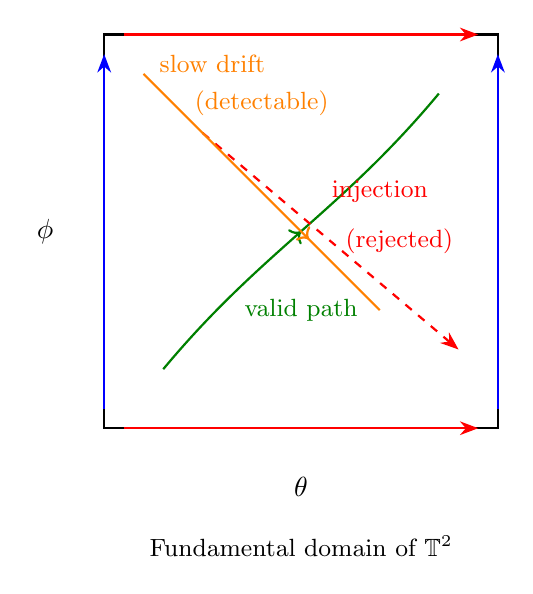
\begin{tikzpicture}[scale=2.5]
    % Draw torus representation as a square with identified edges
    \draw[thick] (0,0) rectangle (2,2);

    % Arrows indicating identification
    \draw[-{Stealth},thick,blue] (0,0.1) -- (0,1.9);
    \draw[-{Stealth},thick,blue] (2,0.1) -- (2,1.9);
    \draw[-{Stealth},thick,red] (0.1,0) -- (1.9,0);
    \draw[-{Stealth},thick,red] (0.1,2) -- (1.9,2);

    % Normal trajectory (smooth curve)
    \draw[thick,green!50!black,decoration={markings,mark=at position 0.5 with {\arrow{>}}},postaction={decorate}]
        (0.3,0.3) .. controls (0.8,0.9) and (1.2,1.1) .. (1.7,1.7);
    \node[green!50!black] at (1.0,0.6) {\small valid path};

    % Injection attempt (sharp jump) - shown as dashed
    \draw[thick,red,dashed,-{Stealth}] (0.5,1.5) -- (1.8,0.4);
    \node[red] at (1.4,1.2) {\small injection};
    \node[red] at (1.5,0.95) {\small (rejected)};

    % Slow drift attack
    \draw[thick,orange,decoration={markings,mark=at position 0.7 with {\arrow{>}}},postaction={decorate}]
        (0.2,1.8) .. controls (0.4,1.6) and (0.6,1.4) .. (0.8,1.2)
        .. controls (1.0,1.0) and (1.2,0.8) .. (1.4,0.6);
    \node[orange] at (0.55,1.85) {\small slow drift};
    \node[orange] at (0.8,1.65) {\small (detectable)};

    % Labels
    \node at (1,-0.3) {$\theta$};
    \node at (-0.3,1) {$\phi$};
    \node at (1,-0.6) {\small Fundamental domain of $\mathbb{T}^2$};
\end{tikzpicture}
\caption{Dynamics on $\mathbb{T}^2$ under coherence constraints. Valid trajectories (green) follow smooth paths with bounded curvature. Impulsive injection attempts (red, dashed) violate energy bounds and are rejected. Slow drift attacks (orange) respect local constraints but require many steps and leave detectable traces.}
\label{fig:torus}
\end{figure}

\section{Coherence Trace Analysis}
\label{sec:traces}

To operationalize detection of residual attacks, we define:

\begin{definition}[Coherence Trace]
A coherence trace is a time-ordered sequence $\tau = \{(z_t, \kappa_t, \Delta H_t, A_t)\}_{t=1}^{T}$ where:
\begin{itemize}
    \item $z_t \in \mathcal{M}$ is the latent state,
    \item $\kappa_t = \|z_{t+1} - 2z_t + z_{t-1}\|$ is local curvature,
    \item $\Delta H_t = H(z_{t+1}) - H(z_t)$ is energy variation,
    \item $A_t = \mathbf{1}[z_{t+1} \notin \mathcal{N}_\delta(z_t)]$ is an adjacency violation flag.
\end{itemize}
\end{definition}

Anomalous trajectories exhibit one or more of:

\begin{enumerate}
    \item \textbf{Curvature spikes}: $\kappa_t > \kappa_{\max}$ indicates attempted discontinuous transition.

    \item \textbf{Sustained drift}: $\sum_{t=1}^{T} \Delta H_t > \epsilon T$ with consistent sign indicates directed displacement.

    \item \textbf{Frequency leakage}: High-frequency spectral components $|\hat{z}_k|$ for $k > k_{\max}$ indicate attempted injection that partially bypassed rejection.

    \item \textbf{Adjacency violations}: $\sum_t A_t > 0$ indicates topological discontinuity.
\end{enumerate}

These signals are computable from the latent trajectory without access to input semantics.

\section{Relation to Existing Methods}
\label{sec:related}

Several existing paradigms involve constraints on generation. Our proposal differs in level of operation and the nature of guarantees.

\subsection{Constrained Decoding}

Methods such as FUDGE \cite{yang2021}, NeuroLogic \cite{lu2021}, and GeLaTo \cite{zhang2023} impose constraints at the token level during autoregressive generation. These operate on:
\begin{itemize}
    \item discrete token sequences,
    \item local next-token distributions,
    \item output-level properties (lexical, syntactic, semantic).
\end{itemize}

\textbf{Distinction}: We propose constraints on continuous latent trajectories, not discrete outputs. Token-level constraints cannot prevent latent displacement that occurs before decoding.

\subsection{Energy-Based Models}

EBMs \cite{lecun2006,du2019} define an energy function over outputs and sample via MCMC or Langevin dynamics. Recent work applies EBMs to text \cite{deng2020,qin2022}.

\textbf{Distinction}: EBMs define energy over \emph{outputs} or \emph{input-output pairs}. We define coherence over \emph{latent state transitions}. An EBM may assign low energy to an adversarially-reached output; our framework would flag the trajectory that reached it.

\subsection{Diffusion Models}

Diffusion models \cite{ho2020,song2021} generate via iterative denoising along a stochastic path. They implicitly define a manifold of reachable outputs.

\textbf{Distinction}: Diffusion paths are stochastic and lack explicit topological invariants. There is no conserved quantity analogous to $H$. Our framework requires deterministic or controlled-stochastic dynamics with verifiable conservation laws.

\subsection{Summary of Distinctions}

\begin{table}[h]
\centering
\begin{tabular}{@{}lccc@{}}
\toprule
\textbf{Method} & \textbf{Level} & \textbf{Constraint Type} & \textbf{Trajectory Verifiable} \\
\midrule
Constrained decoding & Token & Output properties & No \\
Energy-based models & Output & Energy minimization & No \\
Diffusion models & Output & Stochastic path & No \\
\textbf{This work} & Latent state & Topological + dynamical & Yes \\
\bottomrule
\end{tabular}
\caption{Comparison of constraint paradigms. Our approach operates on latent trajectories with verifiable invariants.}
\label{tab:comparison}
\end{table}

\section{Creativity and Discontinuity}

\subsection{The Discontinuity Objection}

Some creative outputs appear to involve discontinuous conceptual jumps. Does requiring continuous latent paths preclude such creativity?

\subsection{Continuity in Higher Dimensions}

Evidence from cognitive science \cite{lake2017,tenenbaum2011} and representation learning \cite{bengio2013,higgins2018} suggests that apparent discontinuities often correspond to continuous paths in sufficiently high-dimensional or appropriately structured latent spaces.

A ``creative leap'' from concept $A$ to concept $B$ may traverse:
\begin{itemize}
    \item intermediate abstractions,
    \item shared structural features,
    \item analogical bridges in representation space.
\end{itemize}

\subsection{Scoped Claim}

We do not claim that all creativity is continuous. We claim:

\begin{quote}
\emph{Creativity sufficient for language generation does not require unbounded latent displacement.}
\end{quote}

This is empirically testable: if a topologically constrained model produces outputs judged as creative by human evaluators, the claim is supported.

\section{Adversarial Adaptation}

\subsection{Limits of the Proposal}

We do not claim that topological constraints eliminate all attacks. Adversaries may attempt:
\begin{itemize}
    \item low-frequency, coherence-preserving drift,
    \item exploitation of regions where $H$ is poorly defined,
    \item attacks on the coherence functional itself.
\end{itemize}

\subsection{What the Framework Provides}

Topological constraints enforce:

\begin{enumerate}
    \item \textbf{Path dependence}: Attacks must follow valid trajectories. There are no shortcuts.

    \item \textbf{Increased attack cost}: Achieving displacement $D$ requires $O(D/\epsilon)$ steps under curvature bound $\epsilon$.

    \item \textbf{Observable signatures}: Coherence traces reveal sustained directional drift, anomalous curvature, or frequency leakage.
\end{enumerate}

Prompt injection becomes a control problem rather than a single-shot exploit. The attacker must solve an optimal control problem under state and path constraints; the defender gains a detection surface.

\section{Architectural Scope}

\subsection{What This Is Not}

This proposal is not:
\begin{itemize}
    \item a patch to existing transformers,
    \item a training-time intervention,
    \item a prompt engineering technique.
\end{itemize}

\subsection{What This Is}

This proposal describes a different design space characterized by:
\begin{itemize}
    \item \textbf{Explicit latent topology}: The manifold $\mathcal{M}$ is specified, not emergent.
    \item \textbf{Coherence-aware dynamics}: Transitions are governed by $H$-preserving rules.
    \item \textbf{Trajectory-level verification}: Security properties are checked on paths, not outputs.
\end{itemize}

\subsection{Bridging Work}

Connecting this framework to existing architectures requires:
\begin{enumerate}
    \item methods for projecting transformer representations onto compact manifolds \cite{nickel2017,mathieu2019},
    \item integration of Hamiltonian or Lagrangian layers \cite{greydanus2019,cranmer2020},
    \item development of efficient coherence monitoring.
\end{enumerate}

This remains future work.

\section{Conclusion}

Prompt injection is not defeated by rules, alignment, or output filtering, but by restoring structure to latent dynamics. We have argued that:

\begin{enumerate}
    \item Injection succeeds due to unconstrained latent topology, not semantic failure.
    \item Compact manifolds with coherence-preserving dynamics mechanically suppress high-frequency adversarial perturbations.
    \item Creative exploration is preserved: unseen regions remain reachable via continuous paths.
    \item Residual attacks become control problems with observable signatures.
\end{enumerate}

The contribution is not a defense mechanism but a reframing. By treating prompt injection as a dynamical control problem arising from topological permissiveness, we identify a class of architectural constraints that change the nature of possible attacks.

\bigskip
\noindent\textbf{Key claim (scoped):} \emph{Unseen regions remain reachable, but only through coherent paths. Restoring topology to latent dynamics transforms prompt injection from exploit to control problem.}

\bibliographystyle{plain}
\begin{thebibliography}{99}

\bibitem{amari2016}
S.~Amari.
\newblock Information Geometry and Its Applications.
\newblock Springer, 2016.

\bibitem{arditi2024}
A.~Arditi et al.
\newblock Refusal in language models is mediated by a single direction.
\newblock \emph{arXiv:2406.11717}, 2024.

\bibitem{arnold1989}
V.~Arnold.
\newblock Mathematical Methods of Classical Mechanics.
\newblock Springer, 2nd edition, 1989.

\bibitem{bai2022}
Y.~Bai et al.
\newblock Constitutional AI: Harmlessness from AI feedback.
\newblock \emph{arXiv:2212.08073}, 2022.

\bibitem{belkin2006}
M.~Belkin, P.~Niyogi, and V.~Sindhwani.
\newblock Manifold regularization: A geometric framework for learning from labeled and unlabeled examples.
\newblock \emph{JMLR}, 7:2399--2434, 2006.

\bibitem{bengio2013}
Y.~Bengio, A.~Courville, and P.~Vincent.
\newblock Representation learning: A review and new perspectives.
\newblock \emph{IEEE TPAMI}, 35(8):1798--1828, 2013.

\bibitem{berger1971}
M.~Berger.
\newblock Eigenvalues of the Laplacian.
\newblock In \emph{Global Analysis}, Proc.\ Symp.\ Pure Math., 1971.

\bibitem{chung1997}
F.~Chung.
\newblock Spectral Graph Theory.
\newblock AMS, 1997.

\bibitem{cranmer2020}
M.~Cranmer et al.
\newblock Lagrangian neural networks.
\newblock \emph{ICLR Workshop on Integration of Deep Neural Models and Differential Equations}, 2020.

\bibitem{deng2020}
Y.~Deng et al.
\newblock Residual energy-based models for text generation.
\newblock \emph{ICLR}, 2020.

\bibitem{du2019}
Y.~Du and I.~Mordatch.
\newblock Implicit generation and generalization in energy-based models.
\newblock \emph{NeurIPS}, 2019.

\bibitem{greshake2023}
K.~Greshake et al.
\newblock Not what you've signed up for: Compromising real-world LLM-integrated applications with indirect prompt injection.
\newblock \emph{arXiv:2302.12173}, 2023.

\bibitem{greydanus2019}
S.~Greydanus, M.~Dzamba, and J.~Yosinski.
\newblock Hamiltonian neural networks.
\newblock \emph{NeurIPS}, 2019.

\bibitem{grigoryan2009}
A.~Grigor'yan.
\newblock Heat Kernel and Analysis on Manifolds.
\newblock AMS, 2009.

\bibitem{higgins2018}
I.~Higgins et al.
\newblock Towards a definition of disentangled representations.
\newblock \emph{arXiv:1812.02230}, 2018.

\bibitem{ho2020}
J.~Ho, A.~Jain, and P.~Abbeel.
\newblock Denoising diffusion probabilistic models.
\newblock \emph{NeurIPS}, 2020.

\bibitem{katok1995}
A.~Katok and B.~Hasselblatt.
\newblock Introduction to the Modern Theory of Dynamical Systems.
\newblock Cambridge University Press, 1995.

\bibitem{khalil2002}
H.~Khalil.
\newblock Nonlinear Systems.
\newblock Prentice Hall, 3rd edition, 2002.

\bibitem{lake2017}
B.~Lake, T.~Ullman, J.~Tenenbaum, and S.~Gershman.
\newblock Building machines that learn and think like people.
\newblock \emph{Behavioral and Brain Sciences}, 40:e253, 2017.

\bibitem{lecun2006}
Y.~LeCun, S.~Chopra, R.~Hadsell, M.~Ranzato, and F.~Huang.
\newblock A tutorial on energy-based learning.
\newblock In \emph{Predicting Structured Data}. MIT Press, 2006.

\bibitem{lu2021}
X.~Lu et al.
\newblock NeuroLogic decoding: (Un)supervised neural text generation with predicate logic constraints.
\newblock \emph{NAACL}, 2021.

\bibitem{lyapunov1892}
A.~Lyapunov.
\newblock The general problem of the stability of motion.
\newblock PhD thesis, Kharkov, 1892. (Reprinted in \emph{Int.\ J.\ Control}, 1992.)

\bibitem{mathieu2019}
E.~Mathieu et al.
\newblock Continuous hierarchical representations with Poincar\'e variational auto-encoders.
\newblock \emph{NeurIPS}, 2019.

\bibitem{miyato2018}
T.~Miyato et al.
\newblock Spectral normalization for generative adversarial networks.
\newblock \emph{ICLR}, 2018.

\bibitem{nickel2017}
M.~Nickel and D.~Kiela.
\newblock Poincar\'e embeddings for learning hierarchical representations.
\newblock \emph{NeurIPS}, 2017.

\bibitem{ouyang2022}
L.~Ouyang et al.
\newblock Training language models to follow instructions with human feedback.
\newblock \emph{NeurIPS}, 2022.

\bibitem{perez2022}
F.~Perez and I.~Ribas.
\newblock Ignore this title and HackAPrompt: Exposing systemic vulnerabilities of LLMs through a global prompt hacking competition.
\newblock \emph{EMNLP}, 2022.

\bibitem{qin2022}
L.~Qin et al.
\newblock Cold decoding: Energy-based constrained text generation with Langevin dynamics.
\newblock \emph{NeurIPS}, 2022.

\bibitem{shuman2013}
D.~Shuman, S.~Narang, P.~Frossard, A.~Ortega, and P.~Vandergheynst.
\newblock The emerging field of signal processing on graphs.
\newblock \emph{IEEE Signal Processing Magazine}, 30(3):83--98, 2013.

\bibitem{song2021}
Y.~Song et al.
\newblock Score-based generative modeling through stochastic differential equations.
\newblock \emph{ICLR}, 2021.

\bibitem{tenenbaum2011}
J.~Tenenbaum, C.~Kemp, T.~Griffiths, and N.~Goodman.
\newblock How to grow a mind: Statistics, structure, and abstraction.
\newblock \emph{Science}, 331(6022):1279--1285, 2011.

\bibitem{wei2023jailbreak}
A.~Wei, N.~Haghtalab, and J.~Steinhardt.
\newblock Jailbroken: How does LLM safety training fail?
\newblock \emph{NeurIPS}, 2023.

\bibitem{yang2021}
K.~Yang and D.~Klein.
\newblock FUDGE: Controlled text generation with future discriminators.
\newblock \emph{NAACL}, 2021.

\bibitem{zhang2023}
H.~Zhang et al.
\newblock GeLaTo: Generative latent textual optimization for text generation.
\newblock \emph{ACL}, 2023.

\bibitem{zou2023}
A.~Zou et al.
\newblock Universal and transferable adversarial attacks on aligned language models.
\newblock \emph{arXiv:2307.15043}, 2023.

\bibitem{cormier2025erlhs}
S.~Cormier.
\newblock ERLHS: A Hamiltonian framework for coherence-preserving machine intelligence.
\newblock \emph{Zenodo}, 2025.
\newblock DOI: \href{https://doi.org/10.5281/zenodo.17928909}{10.5281/zenodo.17928909}.

\bibitem{cormier2026topological}
S.~Cormier.
\newblock Topological constraints for coherent language models: Why geometry prevents hallucination.
\newblock \emph{Paraxiom Research}, 2026.

\end{thebibliography}

\end{document}
